% Needs to be done: electric layout
%                   ltspice simulation
%                   report
%% bare_conf.tex
%% V1.3
%% 2007/01/11
%% by Michael Shell
%% See:
%% http://www.michaelshell.org/
%% for current contact information.
%%
%% This is a skeleton file demonstrating the use of IEEEtran.cls
%% (requires IEEEtran.cls version 1.7 or later) with an IEEE conference paper.
%%
%% Support sites:
%% http://www.michaelshell.org/tex/ieeetran/
%% http://www.ctan.org/tex-archive/macros/latex/contrib/IEEEtran/
%% and
%% http://www.ieee.org/

%%*************************************************************************
%% Legal Notice:
%% This code is offered as-is without any warranty either expressed or
%% implied; without even the implied warranty of MERCHANTABILITY or
%% FITNESS FOR A PARTICULAR PURPOSE! 
%% User assumes all risk.
%% In no event shall IEEE or any contributor to this code be liable for
%% any damages or losses, including, but not limited to, incidental,
%% consequential, or any other damages, resulting from the use or misuse
%% of any information contained here.
%%
%% All comments are the opinions of their respective authors and are not
%% necessarily endorsed by the IEEE.
%%
%% This work is distributed under the LaTeX Project Public License (LPPL)
%% ( http://www.latex-project.org/ ) version 1.3, and may be freely used,
%% distributed and modified. A copy of the LPPL, version 1.3, is included
%% in the base LaTeX documentation of all distributions of LaTeX released
%% 2003/12/01 or later.
%% Retain all contribution notices and credits.
%% ** Modified files should be clearly indicated as such, including  **
%% ** renaming them and changing author support contact information. **
%%
%% File list of work: IEEEtran.cls, IEEEtran_HOWTO.pdf, bare_adv.tex,
%%                    bare_conf.tex, bare_jrnl.tex, bare_jrnl_compsoc.tex
%%*************************************************************************

% *** Authors should verify (and, if needed, correct) their LaTeX system  ***
% *** with the testflow diagnostic prior to trusting their LaTeX platform ***
% *** with production work. IEEE's font choices can trigger bugs that do  ***
% *** not appear when using other class files.                            ***
% The testflow support page is at:
% http://www.michaelshell.org/tex/testflow/

% Note that the a4paper option is mainly intended so that authors in
% countries using A4 can easily print to A4 and see how their papers will
% look in print - the typesetting of the document will not typically be
% affected with changes in paper size (but the bottom and side margins will).
% Use the testflow package mentioned above to verify correct handling of
% both paper sizes by the user's LaTeX system.
%
% Also note that the "draftcls" or "draftclsnofoot", not "draft", option
% should be used if it is desired that the figures are to be displayed in
% draft mode.
%
\documentclass[conference]{IEEEtran}
% Add the compsoc option for Computer Society conferences.
%
% If IEEEtran.cls has not been installed into the LaTeX system files,
% manually specify the path to it like:
% \documentclass[conference]{../sty/IEEEtran}





% Some very useful LaTeX packages include:
% (uncomment the ones you want to load)


% *** MISC UTILITY PACKAGES ***
%
%\usepackage{ifpdf}
% Heiko Oberdiek's ifpdf.sty is very useful if you need conditional
% compilation based on whether the output is pdf or dvi.
% usage:
% \ifpdf
%   % pdf code
% \else
%   % dvi code
% \fi
% The latest version of ifpdf.sty can be obtained from:
% http://www.ctan.org/tex-archive/macros/latex/contrib/oberdiek/
% Also, note that IEEEtran.cls V1.7 and later provides a builtin
% \ifCLASSINFOpdf conditional that works the same way.
% When switching from latex to pdflatex and vice-versa, the compiler may
% have to be run twice to clear warning/error messages.






% *** CITATION PACKAGES ***
%
\usepackage{cite}
% cite.sty was written by Donald Arseneau
% V1.6 and later of IEEEtran pre-defines the format of the cite.sty package
% \cite{} output to follow that of IEEE. Loading the cite package will
% result in citation numbers being automatically sorted and properly
% "compressed/ranged". e.g., [1], [9], [2], [7], [5], [6] without using
% cite.sty will become [1], [2], [5]--[7], [9] using cite.sty. cite.sty's
% \cite will automatically add leading space, if needed. Use cite.sty's
% noadjust option (cite.sty V3.8 and later) if you want to turn this off.
% cite.sty is already installed on most LaTeX systems. Be sure and use
% version 4.0 (2003-05-27) and later if using hyperref.sty. cite.sty does
% not currently provide for hyperlinked citations.
% The latest version can be obtained at:
% http://www.ctan.org/tex-archive/macros/latex/contrib/cite/
% The documentation is contained in the cite.sty file itself.






% *** GRAPHICS RELATED PACKAGES ***
%
\ifCLASSINFOpdf
   \usepackage[pdftex]{graphicx}
  % declare the path(s) where your graphic files are
  % \graphicspath{{../pdf/}{../jpeg/}}
  % and their extensions so you won't have to specify these with
  % every instance of \includegraphics
  % \DeclareGraphicsExtensions{.pdf,.jpeg,.png}
\else
  % or other class option (dvipsone, dvipdf, if not using dvips). graphicx
  % will default to the driver specified in the system graphics.cfg if no
  % driver is specified.
   \usepackage[dvips]{graphicx}
  % declare the path(s) where your graphic files are
  % \graphicspath{{../eps/}}
  % and their extensions so you won't have to specify these with
  % every instance of \includegraphics
  % \DeclareGraphicsExtensions{.eps}
\fi
% graphicx was written by David Carlisle and Sebastian Rahtz. It is
% required if you want graphics, photos, etc. graphicx.sty is already
% installed on most LaTeX systems. The latest version and documentation can
% be obtained at: 
% http://www.ctan.org/tex-archive/macros/latex/required/graphics/
% Another good source of documentation is "Using Imported Graphics in
% LaTeX2e" by Keith Reckdahl which can be found as epslatex.ps or
% epslatex.pdf at: http://www.ctan.org/tex-archive/info/
%
% latex, and pdflatex in dvi mode, support graphics in encapsulated
% postscript (.eps) format. pdflatex in pdf mode supports graphics
% in .pdf, .jpeg, .png and .mps (metapost) formats. Users should ensure
% that all non-photo figures use a vector format (.eps, .pdf, .mps) and
% not a bitmapped formats (.jpeg, .png). IEEE frowns on bitmapped formats
% which can result in "jaggedy"/blurry rendering of lines and letters as
% well as large increases in file sizes.
%
% You can find documentation about the pdfTeX application at:
% http://www.tug.org/applications/pdftex



\usepackage{pbox}
\usepackage{hyperref}
% *** MATH PACKAGES ***
%
\usepackage[cmex10]{amsmath}
% A popular package from the American Mathematical Society that provides
% many useful and powerful commands for dealing with mathematics. If using
% it, be sure to load this package with the cmex10 option to ensure that
% only type 1 fonts will utilized at all point sizes. Without this option,
% it is possible that some math symbols, particularly those within
% footnotes, will be rendered in bitmap form which will result in a
% document that can not be IEEE Xplore compliant!
%
% Also, note that the amsmath package sets \interdisplaylinepenalty to 10000
% thus preventing page breaks from occurring within multiline equations. Use:
%\interdisplaylinepenalty=2500
% after loading amsmath to restore such page breaks as IEEEtran.cls normally
% does. amsmath.sty is already installed on most LaTeX systems. The latest
% version and documentation can be obtained at:
% http://www.ctan.org/tex-archive/macros/latex/required/amslatex/math/





% *** SPECIALIZED LIST PACKAGES ***
%
%\usepackage{algorithmic}
% algorithmic.sty was written by Peter Williams and Rogerio Brito.
% This package provides an algorithmic environment fo describing algorithms.
% You can use the algorithmic environment in-text or within a figure
% environment to provide for a floating algorithm. Do NOT use the algorithm
% floating environment provided by algorithm.sty (by the same authors) or
% algorithm2e.sty (by Christophe Fiorio) as IEEE does not use dedicated
% algorithm float types and packages that provide these will not provide
% correct IEEE style captions. The latest version and documentation of
% algorithmic.sty can be obtained at:
% http://www.ctan.org/tex-archive/macros/latex/contrib/algorithms/
% There is also a support site at:
% http://algorithms.berlios.de/index.html
% Also of interest may be the (relatively newer and more customizable)
% algorithmicx.sty package by Szasz Janos:
% http://www.ctan.org/tex-archive/macros/latex/contrib/algorithmicx/




% *** ALIGNMENT PACKAGES ***
%
%\usepackage{array}
% Frank Mittelbach's and David Carlisle's array.sty patches and improves
% the standard LaTeX2e array and tabular environments to provide better
% appearance and additional user controls. As the default LaTeX2e table
% generation code is lacking to the point of almost being broken with
% respect to the quality of the end results, all users are strongly
% advised to use an enhanced (at the very least that provided by array.sty)
% set of table tools. array.sty is already installed on most systems. The
% latest version and documentation can be obtained at:
% http://www.ctan.org/tex-archive/macros/latex/required/tools/


%\usepackage{mdwmath}
%\usepackage{mdwtab}
% Also highly recommended is Mark Wooding's extremely powerful MDW tools,
% especially mdwmath.sty and mdwtab.sty which are used to format equations
% and tables, respectively. The MDWtools set is already installed on most
% LaTeX systems. The lastest version and documentation is available at:
% http://www.ctan.org/tex-archive/macros/latex/contrib/mdwtools/


% IEEEtran contains the IEEEeqnarray family of commands that can be used to
% generate multiline equations as well as matrices, tables, etc., of high
% quality.


%\usepackage{eqparbox}
% Also of notable interest is Scott Pakin's eqparbox package for creating
% (automatically sized) equal width boxes - aka "natural width parboxes".
% Available at:
% http://www.ctan.org/tex-archive/macros/latex/contrib/eqparbox/





% *** SUBFIGURE PACKAGES ***
\usepackage[tight,footnotesize]{subfigure}
% subfigure.sty was written by Steven Douglas Cochran. This package makes it
% easy to put subfigures in your figures. e.g., "Figure 1a and 1b". For IEEE
% work, it is a good idea to load it with the tight package option to reduce
% the amount of white space around the subfigures. subfigure.sty is already
% installed on most LaTeX systems. The latest version and documentation can
% be obtained at:
% http://www.ctan.org/tex-archive/obsolete/macros/latex/contrib/subfigure/
% subfigure.sty has been superceeded by subfig.sty.



%\usepackage[caption=false]{caption}
%\usepackage[font=footnotesize]{subfig}
% subfig.sty, also written by Steven Douglas Cochran, is the modern
% replacement for subfigure.sty. However, subfig.sty requires and
% automatically loads Axel Sommerfeldt's caption.sty which will override
% IEEEtran.cls handling of captions and this will result in nonIEEE style
% figure/table captions. To prevent this problem, be sure and preload
% caption.sty with its "caption=false" package option. This is will preserve
% IEEEtran.cls handing of captions. Version 1.3 (2005/06/28) and later 
% (recommended due to many improvements over 1.2) of subfig.sty supports
% the caption=false option directly:
%\usepackage[caption=false,font=footnotesize]{subfig}
%
% The latest version and documentation can be obtained at:
% http://www.ctan.org/tex-archive/macros/latex/contrib/subfig/
% The latest version and documentation of caption.sty can be obtained at:
% http://www.ctan.org/tex-archive/macros/latex/contrib/caption/




% *** FLOAT PACKAGES ***
%
\usepackage{fixltx2e}
% fixltx2e, the successor to the earlier fix2col.sty, was written by
% Frank Mittelbach and David Carlisle. This package corrects a few problems
% in the LaTeX2e kernel, the most notable of which is that in current
% LaTeX2e releases, the ordering of single and double column floats is not
% guaranteed to be preserved. Thus, an unpatched LaTeX2e can allow a
% single column figure to be placed prior to an earlier double column
% figure. The latest version and documentation can be found at:
% http://www.ctan.org/tex-archive/macros/latex/base/



%\usepackage{stfloats}
% stfloats.sty was written by Sigitas Tolusis. This package gives LaTeX2e
% the ability to do double column floats at the bottom of the page as well
% as the top. (e.g., "\begin{figure*}[!b]" is not normally possible in
% LaTeX2e). It also provides a command:
%\fnbelowfloat
% to enable the placement of footnotes below bottom floats (the standard
% LaTeX2e kernel puts them above bottom floats). This is an invasive package
% which rewrites many portions of the LaTeX2e float routines. It may not work
% with other packages that modify the LaTeX2e float routines. The latest
% version and documentation can be obtained at:
% http://www.ctan.org/tex-archive/macros/latex/contrib/sttools/
% Documentation is contained in the stfloats.sty comments as well as in the
% presfull.pdf file. Do not use the stfloats baselinefloat ability as IEEE
% does not allow \baselineskip to stretch. Authors submitting work to the
% IEEE should note that IEEE rarely uses double column equations and
% that authors should try to avoid such use. Do not be tempted to use the
% cuted.sty or midfloat.sty packages (also by Sigitas Tolusis) as IEEE does
% not format its papers in such ways.





% *** PDF, URL AND HYPERLINK PACKAGES ***
%
%\usepackage{url}
% url.sty was written by Donald Arseneau. It provides better support for
% handling and breaking URLs. url.sty is already installed on most LaTeX
% systems. The latest version can be obtained at:
% http://www.ctan.org/tex-archive/macros/latex/contrib/misc/
% Read the url.sty source comments for usage information. Basically,
% \url{my_url_here}.





% *** Do not adjust lengths that control margins, column widths, etc. ***
% *** Do not use packages that alter fonts (such as pslatex).         ***
% There should be no need to do such things with IEEEtran.cls V1.6 and later.
% (Unless specifically asked to do so by the journal or conference you plan
% to submit to, of course. )


% correct bad hyphenation here
\hyphenation{op-tical net-works semi-conduc-tor}

%\DeclareMathSizes{ds}{ts}{ss}{sss}, where ds is the display size, ts is the text size, etc.
%\DeclareMathSizes{10}{18}{12}{8} 
%\everymath{\displaystyle}
\begin{document}
%
% paper title
% can use linebreaks \\ within to get better formatting as desired
\title{Bandgap Reference Voltage Project}

\author{\IEEEauthorblockN{Marc Christiansen}
\IEEEauthorblockA{Email: mjch@pdx.edu}\\
\and
\IEEEauthorblockN{Jackson Pugh}
\IEEEauthorblockA{%IEEE Student Member and Officer\\
Email: japugh@pdx.edu}
\and
\IEEEauthorblockN{Krish Ramkumar}
\IEEEauthorblockA{Email: krish13007@gmail.com}}

\maketitle

\begin{abstract}
Write this after the paper has been finished.
\end{abstract}
\IEEEpeerreviewmaketitle

\section{Introduction}
\IEEEPARstart{V}{oltage} references play a critical role in analog and digital circuits.  Fig. \ref{fig:overview} illustrates the relationships between each module found in analog circuits.
\begin{figure}[htb]
  \centering
  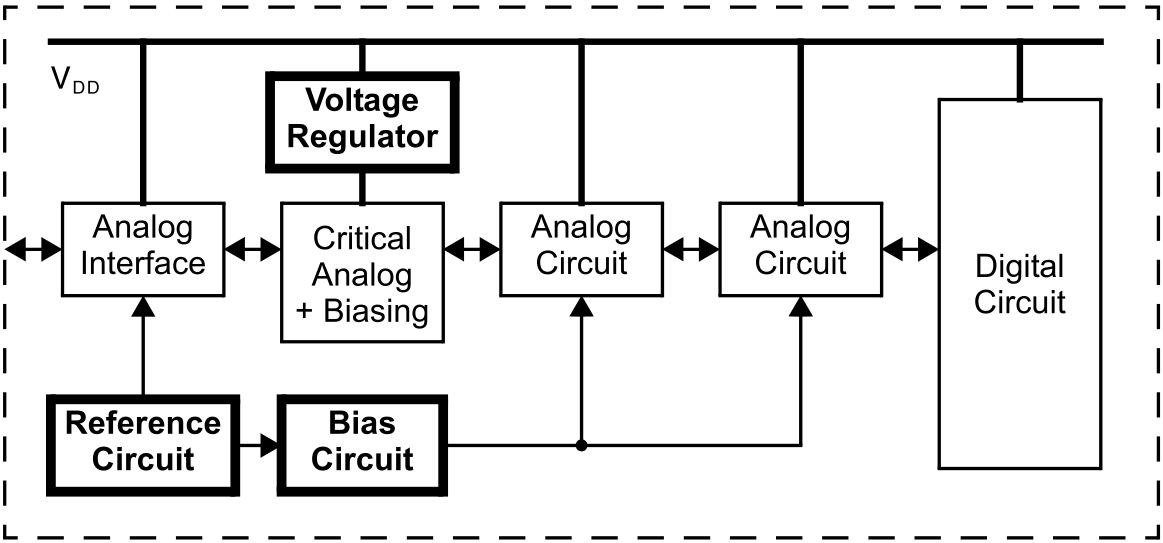
\includegraphics[scale=0.25]{images/overview.png}
  \caption[Overview]{Overview of modules found in analog circuits.\footnotemark}
  \label{fig:overview}
\end{figure}
\footnotetext{Image taken from Analog Integrated Circuit Design 2nd Ed. by Carusone}
\\Ideally, they provide constant voltage regardless of changes in temperature or supply voltage.  This is important for subsystems which depend on a fixed voltage where the environment conditions are not constant.  Examples include ADC/DAC, voltage regulators, and measurement and control systems.
\subsection{Design Tools, Set Up and Assumptions}
The following tools, settings and assumptions were used.
\begin{itemize}
  \item LTspice IV
  \item Electric VLSI Design System
  \item 0.18$\mu$m CMOS technology based off the Analog Integrated Circuit Design 2nd Ed. course website\footnote{\href{http://analogicdesign.com/students/netlists-models/model-files/}{Analog Integrated Circuit Design 2nd Ed. Model Files}} website
  \item Temperature range between -50 to 100 $^\circ$C
  \item Ideal voltage/current source
  \item Ideal operational amplifier
\end{itemize}

\subsection{Objectives}
The main objectives for the voltage reference design are
\begin{enumerate}
  \item Minimize temperature coefficient
  \item Minimize $V_{DD}$ sensitivity
\end{enumerate}
These are achieved through design calculations and using an iterative approach.  The layout is done only for the resistor-MOSFET voltage divider.

\subsection{Design Topologies}
Four different voltage reference topologies are investigated.  %Each design was solved for by hand calculations, modified/iterated for better overall performance, and  simulated and analyzed.
\subsubsection{Design 1. Resistor-MOSFET Voltage Divider}
The most basic design.  It should be good for first-order effects but performance may suffer when higher-order parameters are included.
\subsubsection{Design 2. MOSFET-Only Voltage Divider}
Improved design.  It should have a better temperature coefficient since the P-channel MOSFET load adds an additonal degree of freedom.
\subsubsection{Design 3. Current-Diode Voltage Divider}
Improved design.  It should work extremely well, however the one drawback is the reliance on an ideal current source which is difficult to design.
\subsubsection{Design 4. CMOS Bandgap Voltage Reference}
Advanced design.  Based off the Brokaw Bandgap Reference, this design is implemented using CMOS parasitic BJTs and an ideal operational amplifier.
\subsection{Given parameters}
The following parameters are used in the calculations.
\begin{itemize}
  \item $V_{_{DD}} = 1.8\;\mathrm{V}$
  \item $TC_{_R} = 0.002$
\end{itemize}

\begin{table}[htb]
  \caption{Parameters for calculations}
  \label{tab:parameters}
  \centering
  \begin{tabular}{|l|l|l|}
    \hline
    Parameter                       & NMOS    & PMOS      \\ \hline
    $V_{_{to}}$ (V)                   & 0.45    & -0.45      \\ 
    $K_{_n}$ ($\mu$A/V$^2$)               & 270     & 70         \\ 
    ${\lambda}{\cdot}L$ ($\mu$m/V)  & 0.08    & 0.08       \\ 
    %        ~          & ~    & ~    \\
    \hline
  \end{tabular}
\end{table}

\section{Resistor-MOSFET Voltage Divider}
\subsection{Iteration 1}
Fig. \ref{fig:resistor-mosfet1} shows the schematic for the first iteration.  This is a simple resistor-MOSEFT voltage divider without consideration for loading effects.
\begin{figure}[htb]
  \centering
  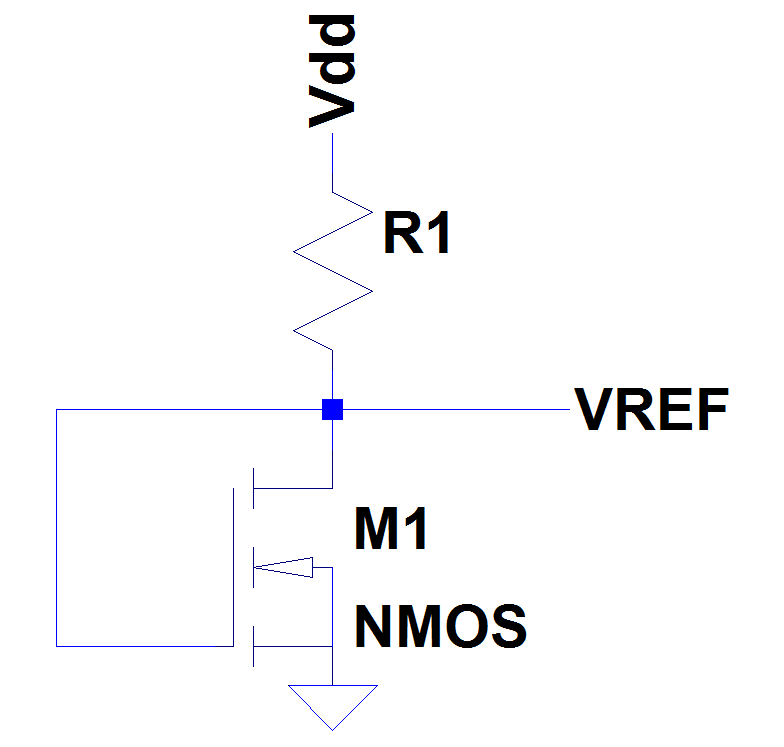
\includegraphics[scale=0.25]{images/resistor-mosfet1.png}
  \caption[resistor1]{Iteration 1 Resistor-MOSFET Circuit}
  \label{fig:resistor-mosfet1}
\end{figure}

\begin{figure}[htb]
  \centering
  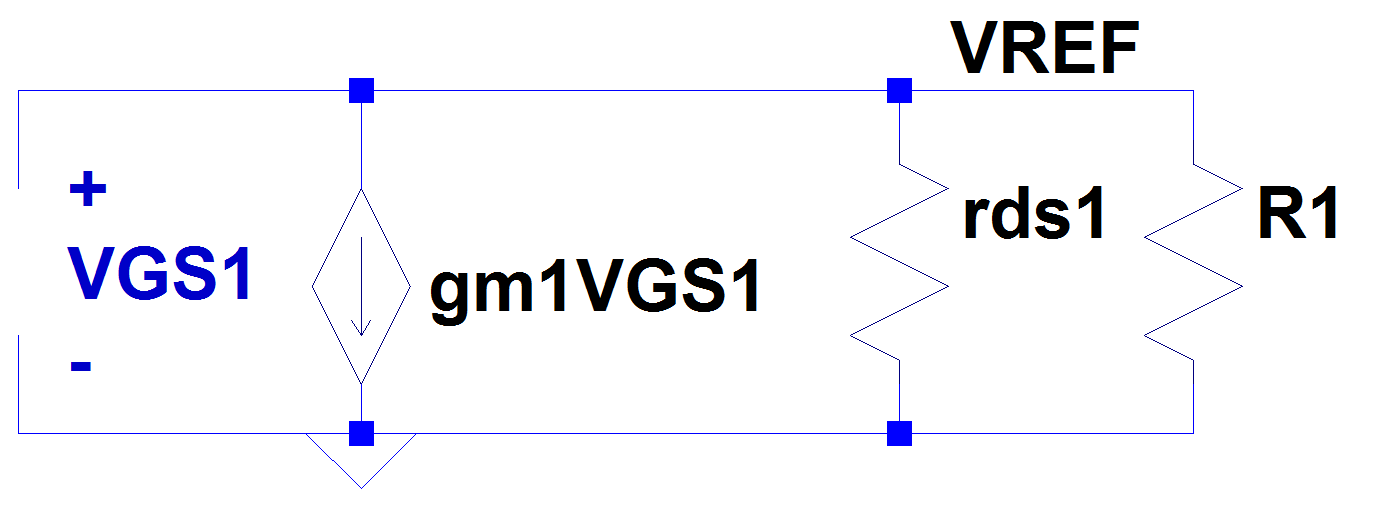
\includegraphics[scale=0.25]{images/resistor-mosfet1-ss.png}
  \caption[resistor1-ss]{Iteration 1 Resistor-MOSFET Small Signal Circuit}
  \label{fig:resistor-mosfet1-ss}
\end{figure}
\subsubsection{Design Equations} 

\begin{table}[ht]
  \caption{Design equations}
  \label{tab:designequations}
  \centering
  \begin{tabular}{|p{1.35cm}|p{8cm}|}
    \hline
    \pbox{1.5cm}{Voltage\\Reference} &
    \begin{equation}
      \label{r_ref}
      V_{_{REF}} = V_{_{TN}} - \sqrt{\frac{2(V_{_{DD}}-V_{_{REF}})}{RK_{_n}}}
    \end{equation}\\
    \hline
    \pbox{1.5cm}{$V_{_{DD}}$\\Sensitivity} &
      \begin{IEEEeqnarray}{rCl}
        \label{r_sensitivity}
        S_{_{VDD}}^{^{V{REF}}} & = & \frac{V_{_{DD}}}{V_{_{REF}}}\frac{\partial{V_{_{REF}}}}{\partial{V_{_{DD}}}}
        \nonumber\\
        & \approx & \frac{1}{V_{_{TN}}\sqrt{\frac{2RK_{_n}}{V_{_{DD}}}}+2}
        \IEEEyesnumber
      \end{IEEEeqnarray}\\
    \hline
    Temperature Coefficient &
    \begin{multline}
      \label{r_tc}
      TC_{_{REF}} = \frac{1}{V_{_{REF}}}\frac{\partial{V_{_{REF}}}}{\partial{T}} =\\\frac{1}{V_{_{REF}}}\left[V_{_{TN}}TC_{_{TN}}-\frac{1}{2}\sqrt{\frac{2L}{W}\frac{V_{_{DD}}}{RKP(T)}}{\cdot}\left[\frac{1}{R}{\cdot}\frac{{\partial}R}{{\partial}T}-\frac{1.5}{T}\right]\right]
    \end{multline}\\
    \hline
  \end{tabular}
\end{table}

\subsection{Iteration 2}
Fig. \ref{fig:resistor-mosfet2} adds an ideal buffer to the output to shield the circuit from loading effectst and leakage current.  Note: These assumptions are also used in Iteration 1 so there are no changes in the calculations.
\subsubsection{Design Equations}
Same as Iteration 1.

\section{MOSFET-Only Voltage Divider}
\subsection{Iteration 1}
\subsubsection{Design Equations}
Analyzing the small-circuit model, 

\begin{figure}[htb]
  \centering
  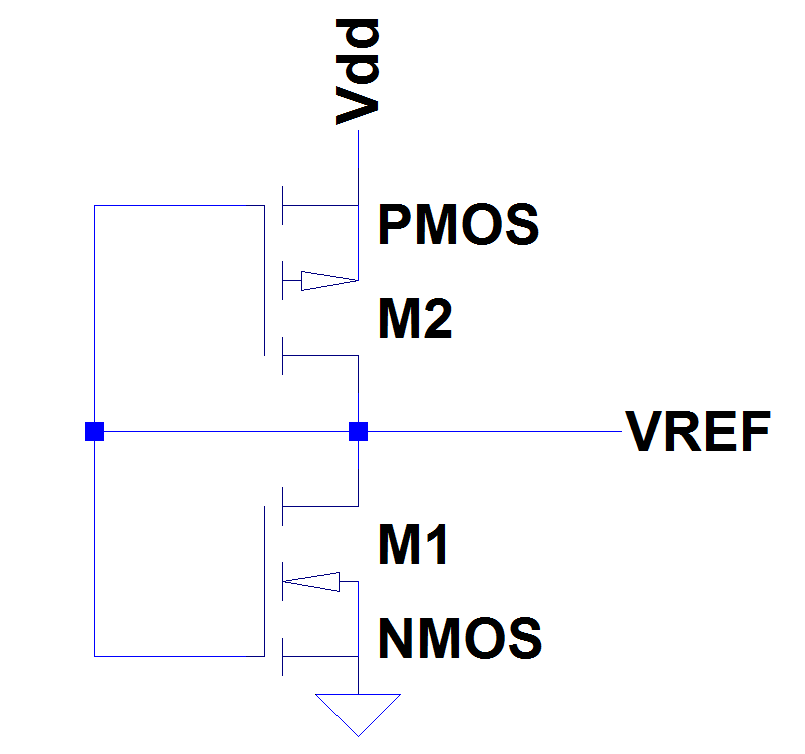
\includegraphics[scale=0.25]{images/mosfet-only1.png}
  \caption[mosfet-only1]{Iteration 1 MOSFET-Only Circuit}
  \label{fig:mosfet-only1}
\end{figure}

\begin{figure}[htb]
  \centering
  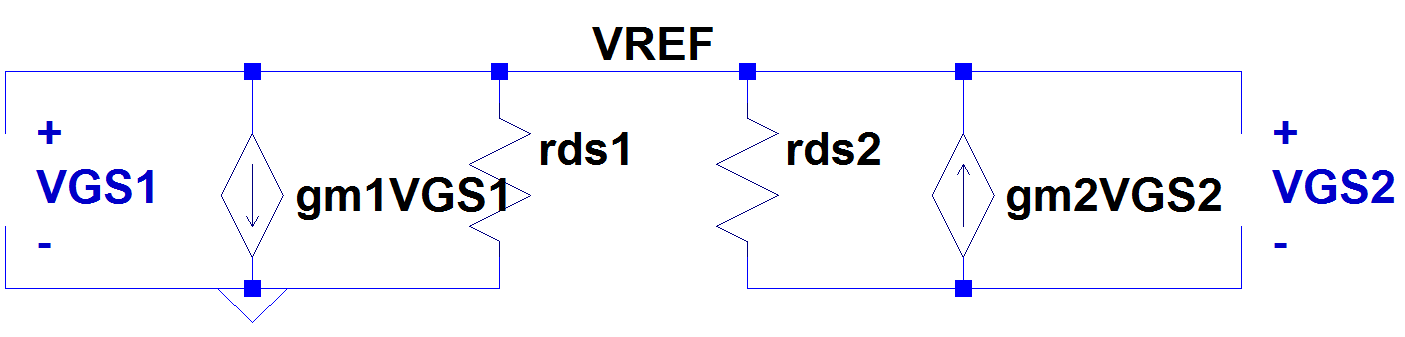
\includegraphics[scale=0.25]{images/mosfet-only1-ss.png}
  \caption[mosfet-only1-ss]{Iteration 1 MOSFET-Only Small Signal Circuit}
  \label{fig:mosfet-only1-ss}
\end{figure}
\begin{equation}
  V_{_{GS1}} = V_{_{GS2}} = V_{_T}
\end{equation}
\begin{IEEEeqnarray}{rCl}
  I_{_T} & = & gm_{_1}V_{_{GS1}} + \frac{V_{_T}}{r_{_{ds1}}} + \frac{V_{_T}}{r_{_{ds2}}} + - gm_{_2}V_{_{GS2}}
  \IEEEyessubnumber\\
  & = & \frac{V_{_T}}{r_{_{ds1}}} + \frac{V_{_T}}{r_{_{ds2}}}
  \nonumber\\
  & = & V_{_T}\left(\frac{1}{r_{_{ds1}}} + \frac{1}{r_{_{ds2}}}\right)
  \IEEEyessubnumber
\end{IEEEeqnarray}
Rearranging for the resistance gives
\begin{IEEEeqnarray}{rCl}
  \frac{V_{_T}}{I_{_T}} & = & \left(\frac{1}{r_{_{ds1}}} + \frac{1}{r_{_{ds2}}}\right)^{-1}
  \nonumber\\
  & = & r_{_{ds1}}//r_{_{ds2}}
  \IEEEyesnumber
\end{IEEEeqnarray}

\begin{IEEEeqnarray}{rCl}
  I_{_{DN}} & = & K_{_n}\left(V_{_{REF}}-V_{_{TN}}\right)^2
  \IEEEyessubnumber\\
  I_{_{DP}} & = & K_{_p}\left(V_{_{REF}}-V_{_{TP}}\right)^2
  \IEEEyessubnumber
\end{IEEEeqnarray}

\begin{equation}
  V_{_{REF}} = \frac{-V_{_{TP}} + V_{_{DD}} + \sqrt{\frac{K_{_n}}{K_{_p}}}V_{_{TN}}}{\sqrt{\frac{K_{_n}}{K_{_p}}} + 1}
\end{equation}

\begin{multline}
  TC(V_{_{REF}}) = \frac{1}{V_{_{REF}}}\frac{{\partial}V_{_{REF}}}{{\partial}T}\\
  = \frac{1}{V_{_{REF}}}\frac{1}{\sqrt{\frac{K_{_n}}{K_{_p}}}+1}\left(\frac{{\partial}-V_{_{TP}}}{{\partial}T} + \sqrt{\frac{K_{_n}}{K_{_p}}}\frac{{\partial}V_{_{TN}}}{{\partial}T}\right)
\end{multline}

\subsection{Iteration 2}
\subsubsection{Design Equations}

\section{Current-Diode Voltage Divider}
\begin{figure}[htb]
  \centering
  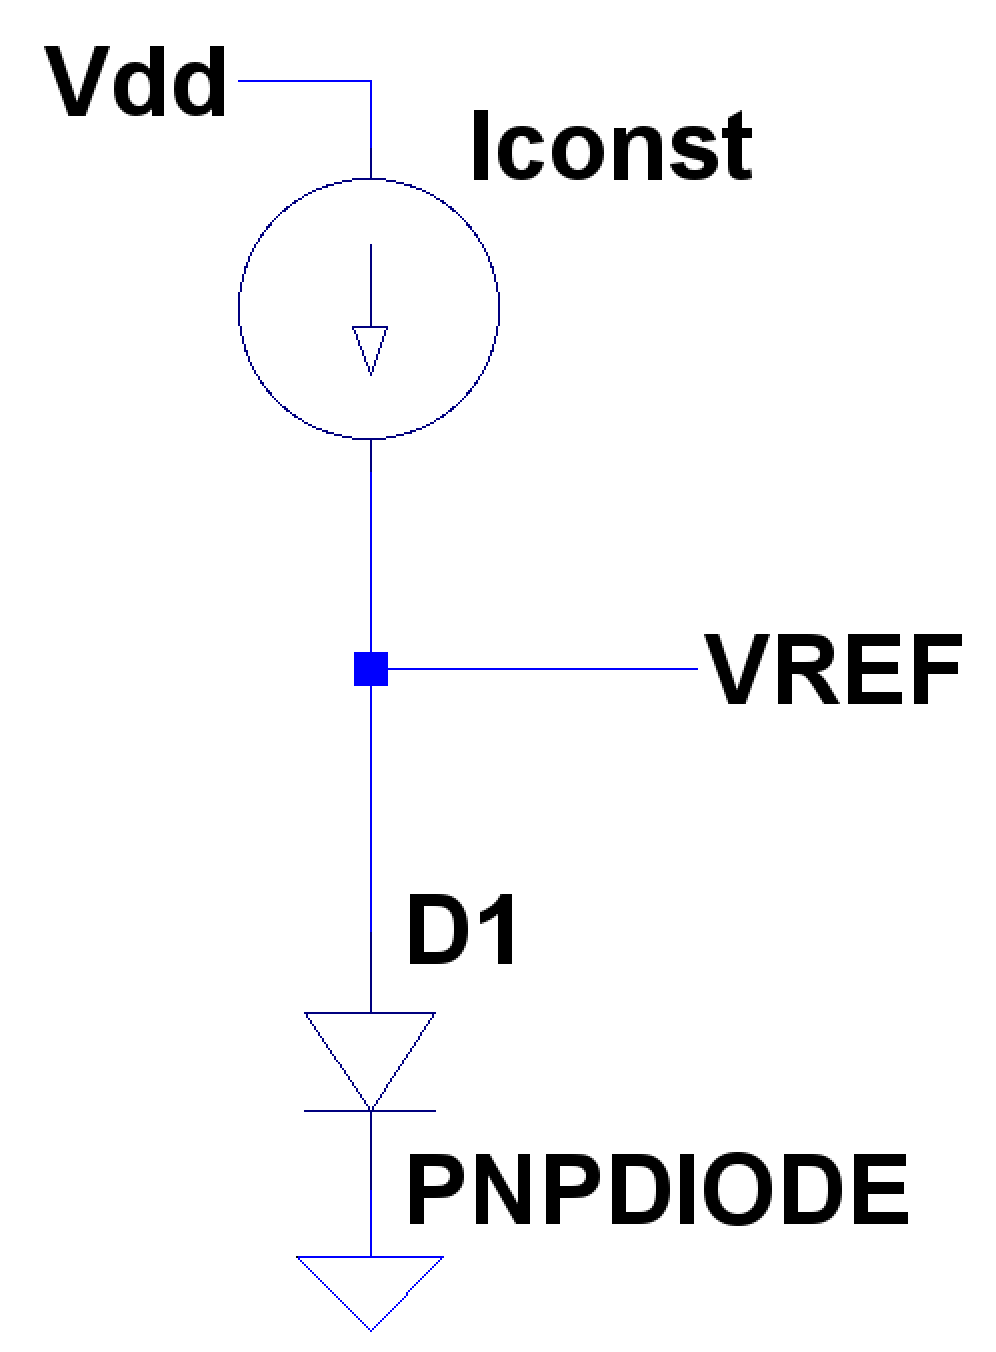
\includegraphics[scale=0.25]{images/cm-diode1.png}
  \caption[cm-diode1]{Iteration 1 Current-Diode Circuit}
  \label{fig:cm-diode1}
\end{figure}
\subsection{Iteration 1}
\subsubsection{Design Equations}

Low frequency small-signal
\begin{equation}
  r_{_d} = \frac{V_{_T}}{I_{_D}} = \frac{kT}{I_{_D}}
\end{equation}
\begin{equation}
  \frac{V_{_T}}{I_{_T}} = \infty = R_{_{in}}
\end{equation}
\begin{equation}
  \frac{V_{_T}}{I_{_T}} = r_{_d} = R_{_{out}}
\end{equation}

\begin{equation}
  I_{_D} = I_se^{^{V_{_D}/V_{T}}} = I_se^{^{qV_{_D}/kT}}
\end{equation}

\begin{equation}
  V_{_{BE0}} = \frac{kT_{_0}ln(I_{_D}/I_s)}{q}
\end{equation}
\begin{multline}
  V_{_{BE}} = V_{_{G0}}(1 - T/T_{_0}) + V_{_{BE0}}T/T_{_0}\\+ \frac{mkT}{q}ln(\frac{T_{_0}}{T}) + \frac{kT}{q}ln(\frac{J_{_c}}{J_{_{c0}}}) 
\end{multline}

\subsection{Iteration 2}
\subsubsection{Design Equations}

\section{CMOS Bandgap Voltage Reference}
\subsection{Iteration 1}
\subsubsection{Design Equations}

\subsection{Iteration 2}
\subsubsection{Design Equations}

\section{Simulation and Results/Conclusions}

\section{Conclusion}
The conclusion goes here.
% conference papers do not normally have an appendix

% use section* for acknowledgement
%\section*{Acknowledgment}
%The authors would like to thank...
% trigger a \newpage just before the given reference
% number - used to balance the columns on the last page
% adjust value as needed - may need to be readjusted if
% the document is modified later
%\IEEEtriggeratref{8}
% The "triggered" command can be changed if desired:
%\IEEEtriggercmd{\enlargethispage{-5in}}

% references section

% can use a bibliography generated by BibTeX as a .bbl file
% BibTeX documentation can be easily obtained at:
% http://www.ctan.org/tex-archive/biblio/bibtex/contrib/doc/
% The IEEEtran BibTeX style support page is at:
% http://www.michaelshell.org/tex/ieeetran/bibtex/
%\bibliographystyle{IEEEtran}
% argument is your BibTeX string definitions and bibliography database(s)
%\bibliography{IEEEabrv,../bib/paper}
%
% <OR> manually copy in the resultant .bbl file
% set second argument of \begin to the number of references
% (used to reserve space for the reference number labels box)
\begin{thebibliography}{1}
\bibitem{IEEEhowto:cmos_baker}
R. Jacob Baker, "CMOS: Circuit Design, Layout, and Simulation", 3rd edition, Wiley-IEEE Press, 2010

\bibitem{IEEEhowto:analog_carusone}
T. Chan Carusone, D. Johns, and K. Martin, "Analog Integrated Circuit Design," 2nd edition, J. Wiley \& Sons, 2011.
\end{thebibliography}
\end{document}
